 % -*- root: ../medieninformatik-arbeit.tex -*-
\documentclass[../medieninformatik-arbeit.tex]{subfiles}
\begin{document}
\section{Implementation}
\label{ch:configurator}
The implementation of the activity sculpture configurator and the activity sculpture were undertaken in a period of around two months. The developed web configurator in this work makes use of cutting edge technologies for both web development and 3D visualization. This project is a demonstration of the capabilities of current web technologies that allow the developing of fully functional data visualization systems that offer integration with other web services for data interchange and support real time interactive 3D visualization.

This chapter will discuss all aspects of the technical implementation of the prototypes discussed in chapter \ref{ch:proto}. The technical requirements for the system will be discussed in the first section followed by an overview of the used technologies. Further on the modules conforming the system and their relationship will be explained in the architecture section. THe configurator section covers the implementation of the controls used by the user to manipulate the sculpture and the generation of the sculpture which are the main functionalities covered in the front end side of the application. The integration of the Whithings API and the manipulation performed on the received data are covered in the backend section of the chapter. Finally an overview of the challenges encountered while developing the system is presented. 

\subsection{Requirements}
Through the analysis of current works described in chapter \ref{ch:related},the requirements of the prototypes in chapter \ref{ch:proto} and in view of the forthcoming user study the functionality and technical requirements of the web-based activity sculpture creator were formulated as follows.

\begin{itemize}
	\item Implement the designed configurator workflow views
	\item Users have to be able to login with their personal Withings account
	\item Query user's data with the Withings API
	\item Store user's data and profile information in a data base
	\item Implement user interface control widgets like buttons, sliders and toggles for the customization area of the configurator
	\item Implement the designed activity sculpture geometry
	\item The visualization of the sculpture has to be rendered in real time  
	\item Changes made in the configurator have to be reflected in the sculpture instantly. avoid the use of update buttons 
	\item Users have to be able to navigate the sculpture in 3D space through rotation and zooming interactions
	\item STL file export support for 3D printing
	\item Support for current browsers
	\item Deployment of a fully working version in a web server for the general public. Anybody with a Withings account should be able to use it an visualize their data.
\end{itemize}


The required functionality is beyond what it would be needed for a basic working prototype. The developed configurator in this work is a fully functional system that fulfills every requirement specified in this section. The stated requirements involved the implementation of other functionality to ensure the requirement was fulfilled. For example the login functionality implies the implementation of an Oauth authentication solution(explained later in section \ref{sub:ApiIntegration}) in order to integrate with the Withings API. Also because the configurator is dealing with personal data the security of the system is important, as a basic approach to address this, the configurator implements session handling.

In the following section the used technologies to tackle the extensive list of requirements will be presented.  

\subsection{Technology}
The web configurator was developed with a modern stack of technologies that enable the use of the JavaScript language not only for frontend but also for the backend, the database and graphics programming. The MEAN stack is a collection of technologies that enables developers to write web applications in a single programming language. MEAN is the acronym for the technologies  conforming the stack: \textit{MongoDB}\cite{mongodb}, \textit{Express}\cite{express}, \textit{AngularJS}\cite{angular} and \textit{Node.js}\cite{joyent2015node}. The acronym was first used by Valeri Karpov, MongoDB engineer, in a blog post\cite{meanstack} where he discussed the benefits of using the same language across all technologies involved. Among the benefits Karpov states their team have experienced an increment in the performance of the developed software and also in the team's productivity. In short the MEAN stack's frameworks will be introduced. 

\textbf{MongoDB} is an ``open-source, document database designed for ease of development and scaling''\cite{mongodb}. Document based are conformed of collections (the equivalent of tables) which can contain several documents (rows) that  to any schema are in essence JSON Objects (JavaScript Object Notation). MongoDB does not enforce any schema to the stored data, making it a very flexible environment to work with. In MongoDB queries are performed in JavaScript providing a seamless integration of the JavaScript language, from querying the information to structuring it in JSON objects. The stored JSON objects are encoded to the BSON format which stands for Binary JSON to enhance efficiency and provide additional data types. Even though working with a schema-less database brings great flexibility, it is recommendable to bring some consistency to the MongoDB documents. For this purpose an object modeling library called \textit{mongoose}\cite{mongoose} has found broad adoption in the developer community. Mongoose provides functionality to easily model the application's data with type casting, custom query functions and other niceties. To illustrate how a mongoose schema looks like, listing \ref{list:mongoose-schema} shows an excerpt of the user schema designed for the configurator.

\begin{lstlisting}[style=htmlcssjs, caption={An excerpt of the user mongoose schema},label=list:mongoose-schema]
// load the mongoose module
var mongoose = require('mongoose');
var Schema = mongoose.Schema;

var userSchema = new Schema({
  profile: {
    name: String, //data type definition
    gender: Number,
    age: Number,
    location: String
  },
// more fields... 
  settings: {
    startDate: Date,
    endDate: Date,
    show: Boolean
  },
  sculptures: {type: Array, "default": []}
});
\end{lstlisting} 

\textbf{Node.js}\cite{joyent2015node} and \textbf{Express}\cite{express} are the frameworks used to develop the web server of the application. Node.js is backend JavaScript, based on the ``V8'' chrome JavaScript runtime providing an event-driven architecture and non-blocking i/o allowing for high performance real time applications. \textit{Node.js} is conformed of basic modules that provide network functionality but it requires the developer to build everything from the ground up. To address this issue the JavaScript library \textit{Express} was developed. Express provides a rich set of features like routing, middleware support and HTTP utilities that allow rapid development of network applications. Listing \ref{list:node-server} shows how a simple server is implemented with Node.js and Express.

\begin{lstlisting}[style=htmlcssjs, caption={Basic Node.js and Express server example},label=list:node-server]
var express = require('express');
var app = express();

app.get('/', function (req, res) {
  res.send('Hello World!');
});

var server = app.listen(3000, function () {
  var host = server.address().address;
  var port = server.address().port;
  console.log('Example app listening at http://%s:%s', host, port);
});
\end{lstlisting}

\textbf{AngularJS}\cite{angular} is the fronted framework in the MEAN stack. \textit{AngularJS} is an opens-source project developed by Google for the development of Single Page Applications (SPAs) where the whole content of a web page is rendered in a single web page and the content is either completely loaded at the beginning or its injected according to user interactions. AngularJS is based on a Model-View-Whatever design pattern (MVW) that allows developers to choose the design pattern that better accommodates their coding style. Whichever design pattern is chosen, AngularJS enforces developers to structure code into modules providing a strong organization in the code base. The functionality provided by AngularJS ranges from bidirectional data-binding, routing, form validation, server communication tools and directives that allow the creation of custom HTML syntax. With frameworks like AngularJS SPA allow to take much of the server workload to the frontend. Another feature of AngularJS is its extensibility. For the purposes of this work the \textit{Angular Material}\cite{angularmaterial} was utilized to implement user interface controls and theming. The \textit{Angular-Material} module is also developed by Google and it provides a solid framework for developing user interfaces utilizing the ``Material design'' philosophies. 

The graphic visualization of the sculpture was implemented with the \textit{Threejs}\cite{cabello2010three} library which provides an approachable abstraction of the \textit{WebGL} API. WebGL is a standard that provides hardware accelerated 3D graphics rendering for the web\cite{webgl}. Based on the OpenGL ES 2.0 standard, WebGL allows the development of real time visualizations in JavaScript through the use of the HTML 5 canvas element. \textit{Threejs} offers developer a wide set of tools and abstractions for rapid development of graphic applications in the web. An example of a basic Threejs application is composed of a scene object that contains cameras, lights and mesh objects that will be rendered to the canvas through a WebGL context. Listing \ref{list:threejs-app} provides a basic example of setting up a the renderer and attaching it to the DOM, loading cameras and lights, creating the scene, adding a cube mesh and finally rendering it.

\begin{lstlisting}[style=htmlcssjs, caption={Basic Threejs 3D app example},label=list:threejs-app, float=t]
var camera, scene, renderer;
var geometry, material, mesh;

renderer = new THREE.WebGLRenderer();
renderer.setSize( window.innerWidth, window.innerHeight );
document.body.appendChild( renderer.domElement );

camera = new THREE.PerspectiveCamera( 50, window.innerWidth/window.innerHeight, 1, 10000 );
camera.position.z = 500;

scene = new THREE.Scene();
					
geometry = new THREE.CubeGeometry(200, 200, 200);
material = new THREE.MeshNormalMaterial({shading: THREE.FlatShading});
mesh = new THREE.Mesh(geometry, material);

scene.add( mesh );
renderer.render( scene, camera );
\end{lstlisting}

In the following sections the utilization the benefits of developing with the MEAN stack with other technologies will be highlighted through examples of modules developed for the web configurator. 

\subsection{Architecture}
By using the MEAN stack to develop the web configurator certain architecture decisions are imposed. One being the use of the backend more as a RESTFul web API (Representational State Transfer) for querying data than for requesting the generation of pages. RESTful APIs define a modern architectural model over the HTTP protocol to perform service operations over a system's data\cite{Fielding:2000:PDM:337180.337228}. A great advantage of utilizing RESTful architectures is that it provides good scalability as the backend can be completely decoupled from the client implementation, meaning one backend can be used to provide data to all sorts of clients from web clients to mobile or desktop applications. The configurator's backend is composed of a web service that implements the Withings API for authentication and requesting sensor data, session handling for assuring only logged in users can access the configurator's backend, the user data API that interacts with the MongoDB database to perform CRUD (Create, Read, Update, Delete) operations on the gathered user data and WebSocket communication support. WebSocket is a protocol based on a TCP connection that provides full-duplex communication to client-server applications\cite{fette2011websocket}. The advantage of WebSockets is that it allows servers to push data to clients without being requested. The configurator makes use of WebSockets through the \textit{Socket.io}\cite{socketio} library which implements the use of WebSockets in an event-driven pattern. Third party libraries utilized in the backend are contained in Node.js modules. Figure \ref{fig:architecture} provides an overview of the modules conforming the backend and frontend sides of the configurator.  

\begin{figure}[h]
\captionsetup{width=\textwidth}
\begin{center}
  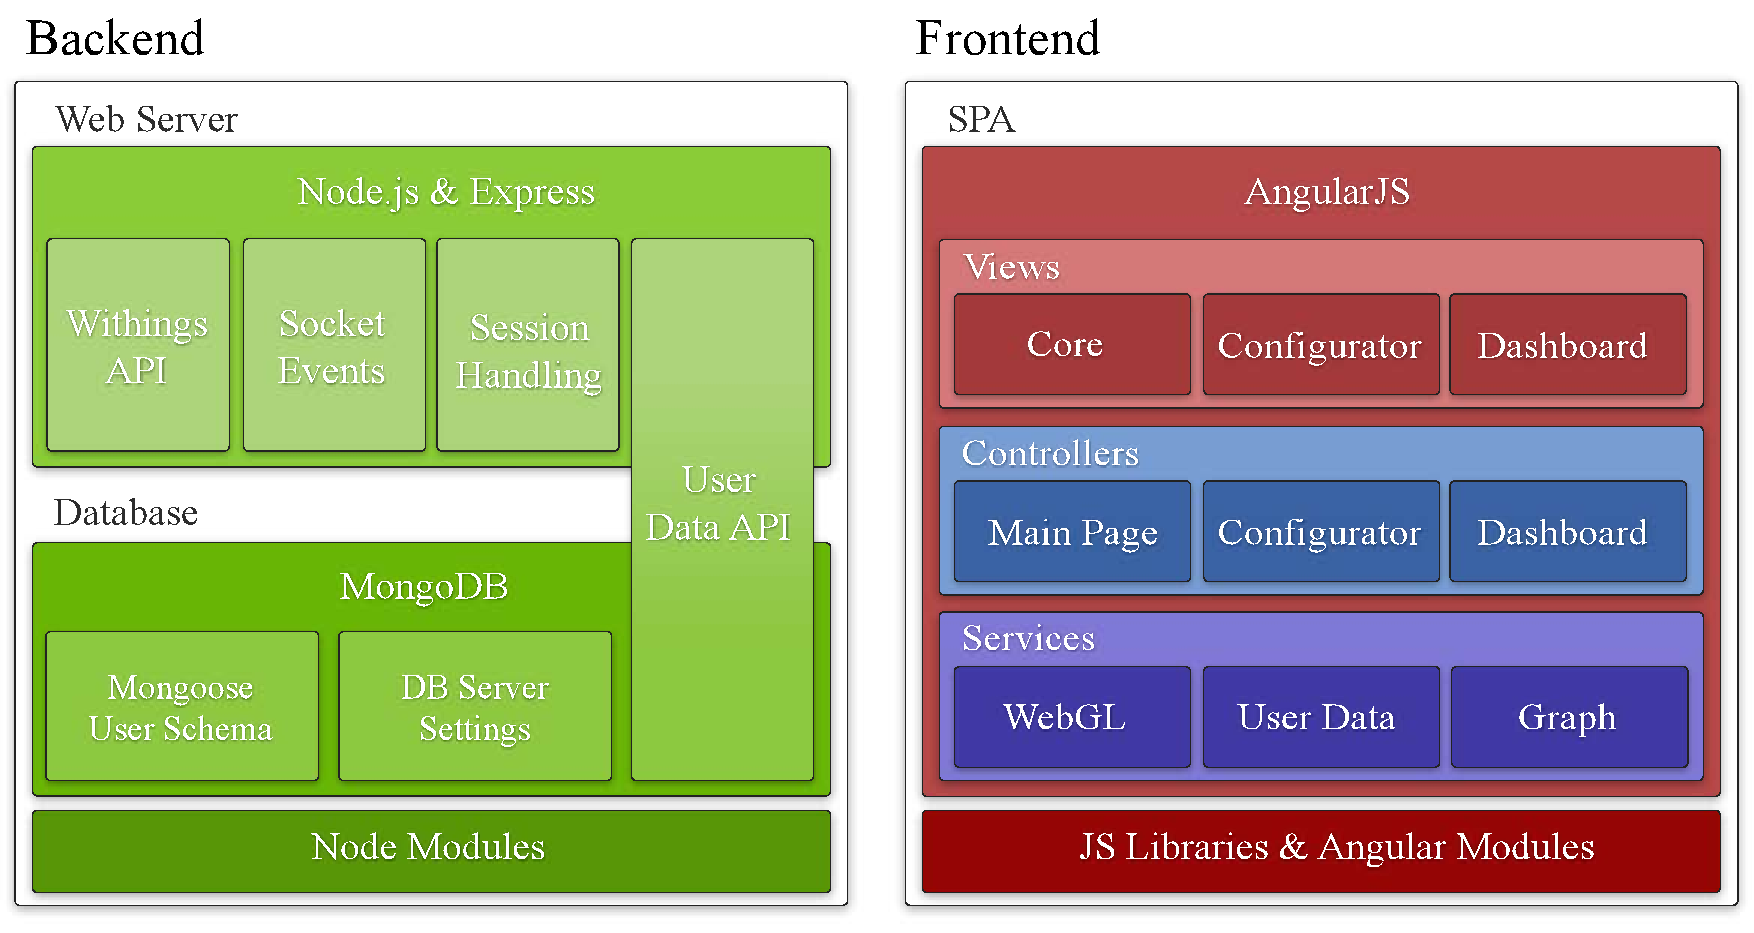
\includegraphics[width=\textwidth]{Configurator/img/Architecture}
  \caption{Activity Sculpture web configurator's architecture}
\label{fig:architecture}
\end{center}
\end{figure}

The frontend of the configurator is a SPA implemented in AngularJS. As discussed before, the backend is implemented as a Web API, relegating the generation of the HTML content to the AngularJS application. The frontend implementation follows a Model View Controller (MVC) pattern for better separation of concerns. Due to the flexibility of AngularJS this is was implemented through the extensive use of controllers attached to views. In AngularJS views are basic HTML templates that describe the visual aspect of the web site. Controllers implement logic functionality to manipulate the application's data or model. The model part of the MVC pattern is implemented by Angular services. Services in Angular are modules that can interface with databases through web APIs or they can be used to abstract functionality and reuse it across the application. Views can host several controllers who at the same time can access several services. 

Even though views in the configurator are divided in several parts for re-usability across the application, they where separated in three main areas: the core, the configurator and the dashboard. The core comprehends partial views utilized for the welcome page, the consent window and the 404 error page. The configurator's view contains several modules with User Interface (UI) controls and the canvas for the sculpture. The dashboard view is composed of the dashboard view that shows the sculpture gallery and charts visualizing the user's data, and the setup form. 

The attached controllers to these views provide the logic to achieve the intention of each section. Due to the specific requirements of each section in the configurator, the controllers are also organized in modules for the main page, the configurator and the dashboard. The main page controller provides the logic for starting the authentication process. The configurator controller is the most complex as it implements the logic the UI controls and the rendering of the sculpture. The configurator controller makes heavy use of the graphics service module, which manages Threejs scenes, cameras and the generation of the sculpture. Further more the configurator controller reaches to the user data service to load the data for the generation of the sculpture. The user data service contains several modules for data manipulation and transforming and provides a user object that holds all the data received from the Withings API. The user object follows a singleton pattern implementation, making a single instance of the object available throughout the application. This is specially helpful as the dashboard configurator also needs the data provided by the user object in order to visualize generate the charts and load the sculpture gallery. For the generation of charts the dashboard controller makes use of a graph service that implements a JavaScript SVG library called \textit{D3.js}\cite{bostock2015d3js}, which stands for ``Data driven documents''. The \textit{D3.js} library has gained broad popularity in web data visualization as it provides great flexibility through data-driven DOM manipulation and the use of widely supported CSS, SVG and JavaScript technologies. 

The router comes next dude!


\begin{figure}[hb!]
\captionsetup{width=\textwidth}
\begin{center}
  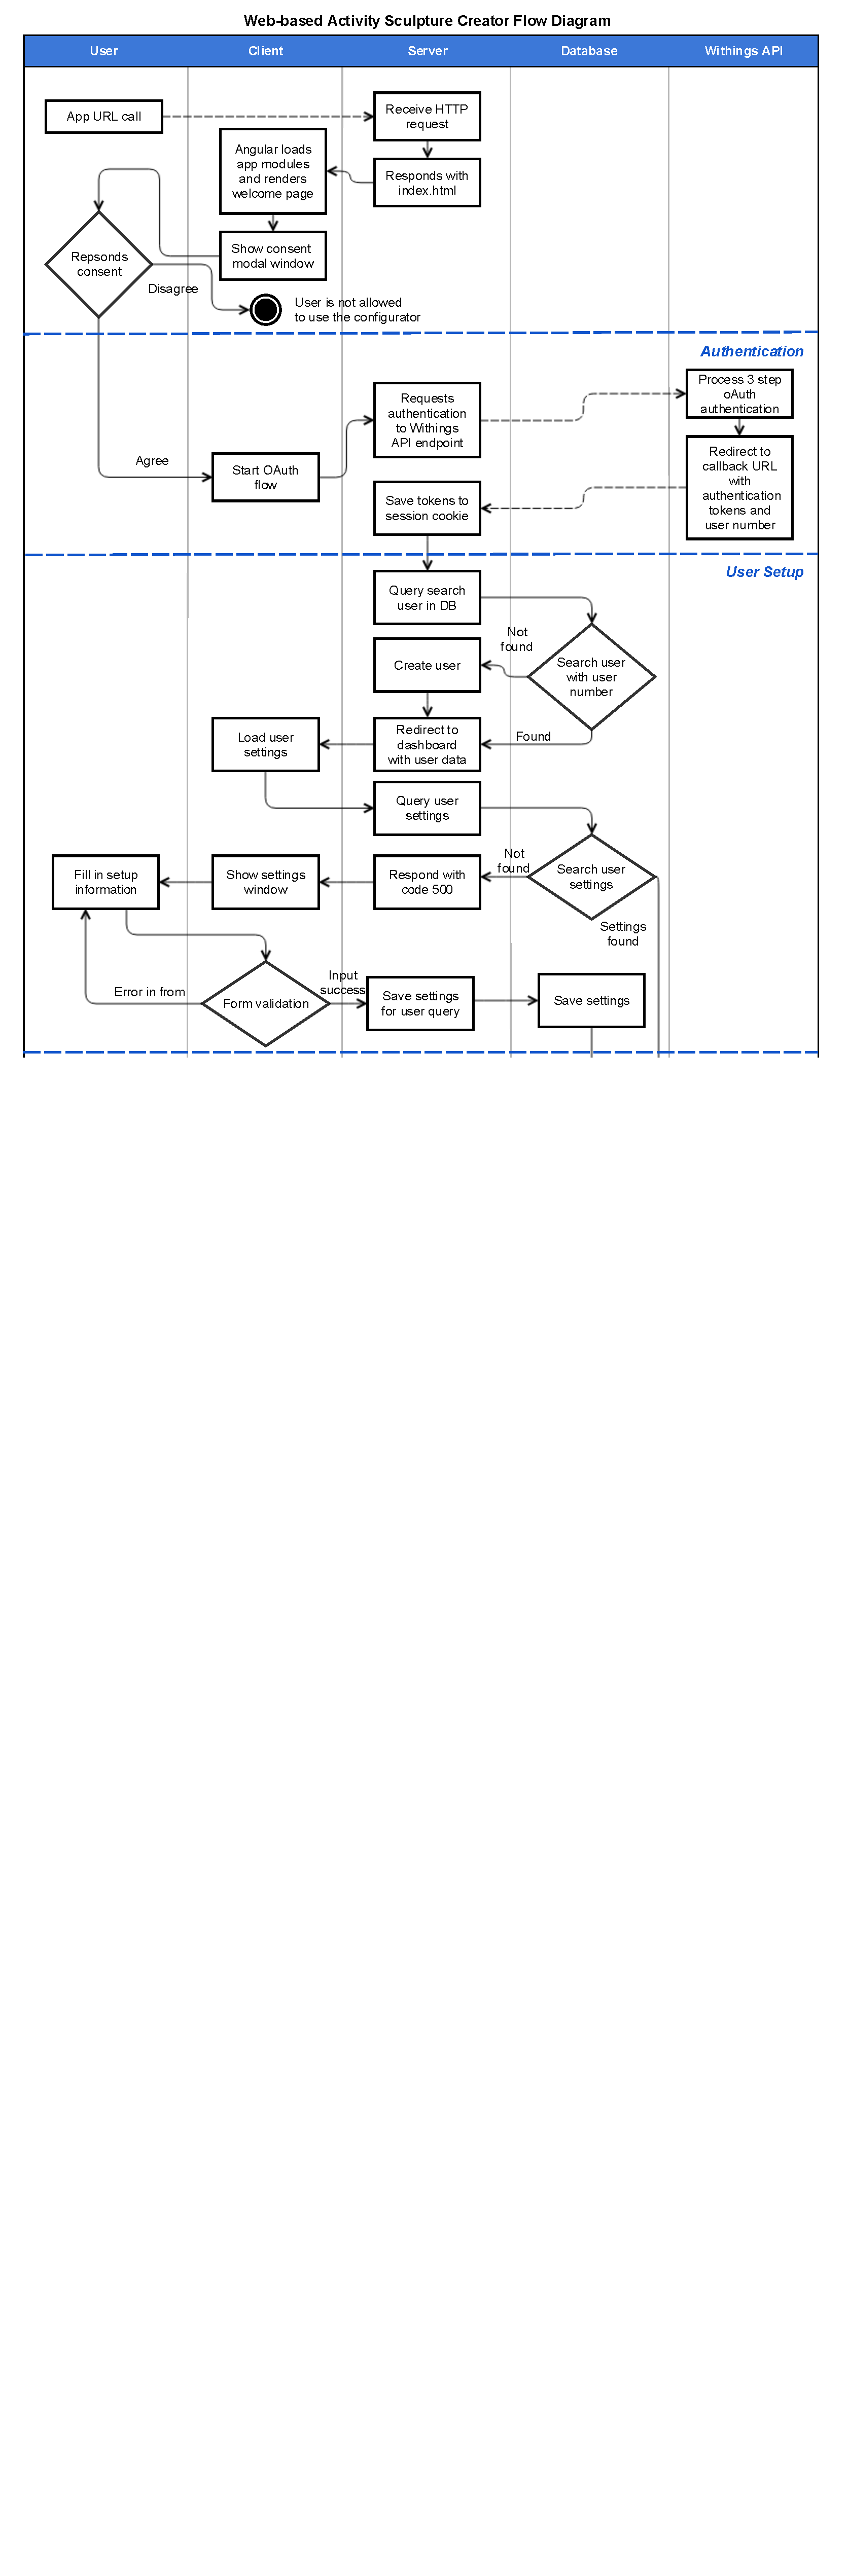
\includegraphics[width=0.82\textwidth]{Configurator/img/flow_diagram_1}
  \caption{Activity Sculpture web configurator's flow diagram part 1}
\label{fig:flowdiagram1}
\end{center}
\end{figure}

\newpage

\begin{figure}[ht!]
\captionsetup{width=\textwidth}
\begin{center}
  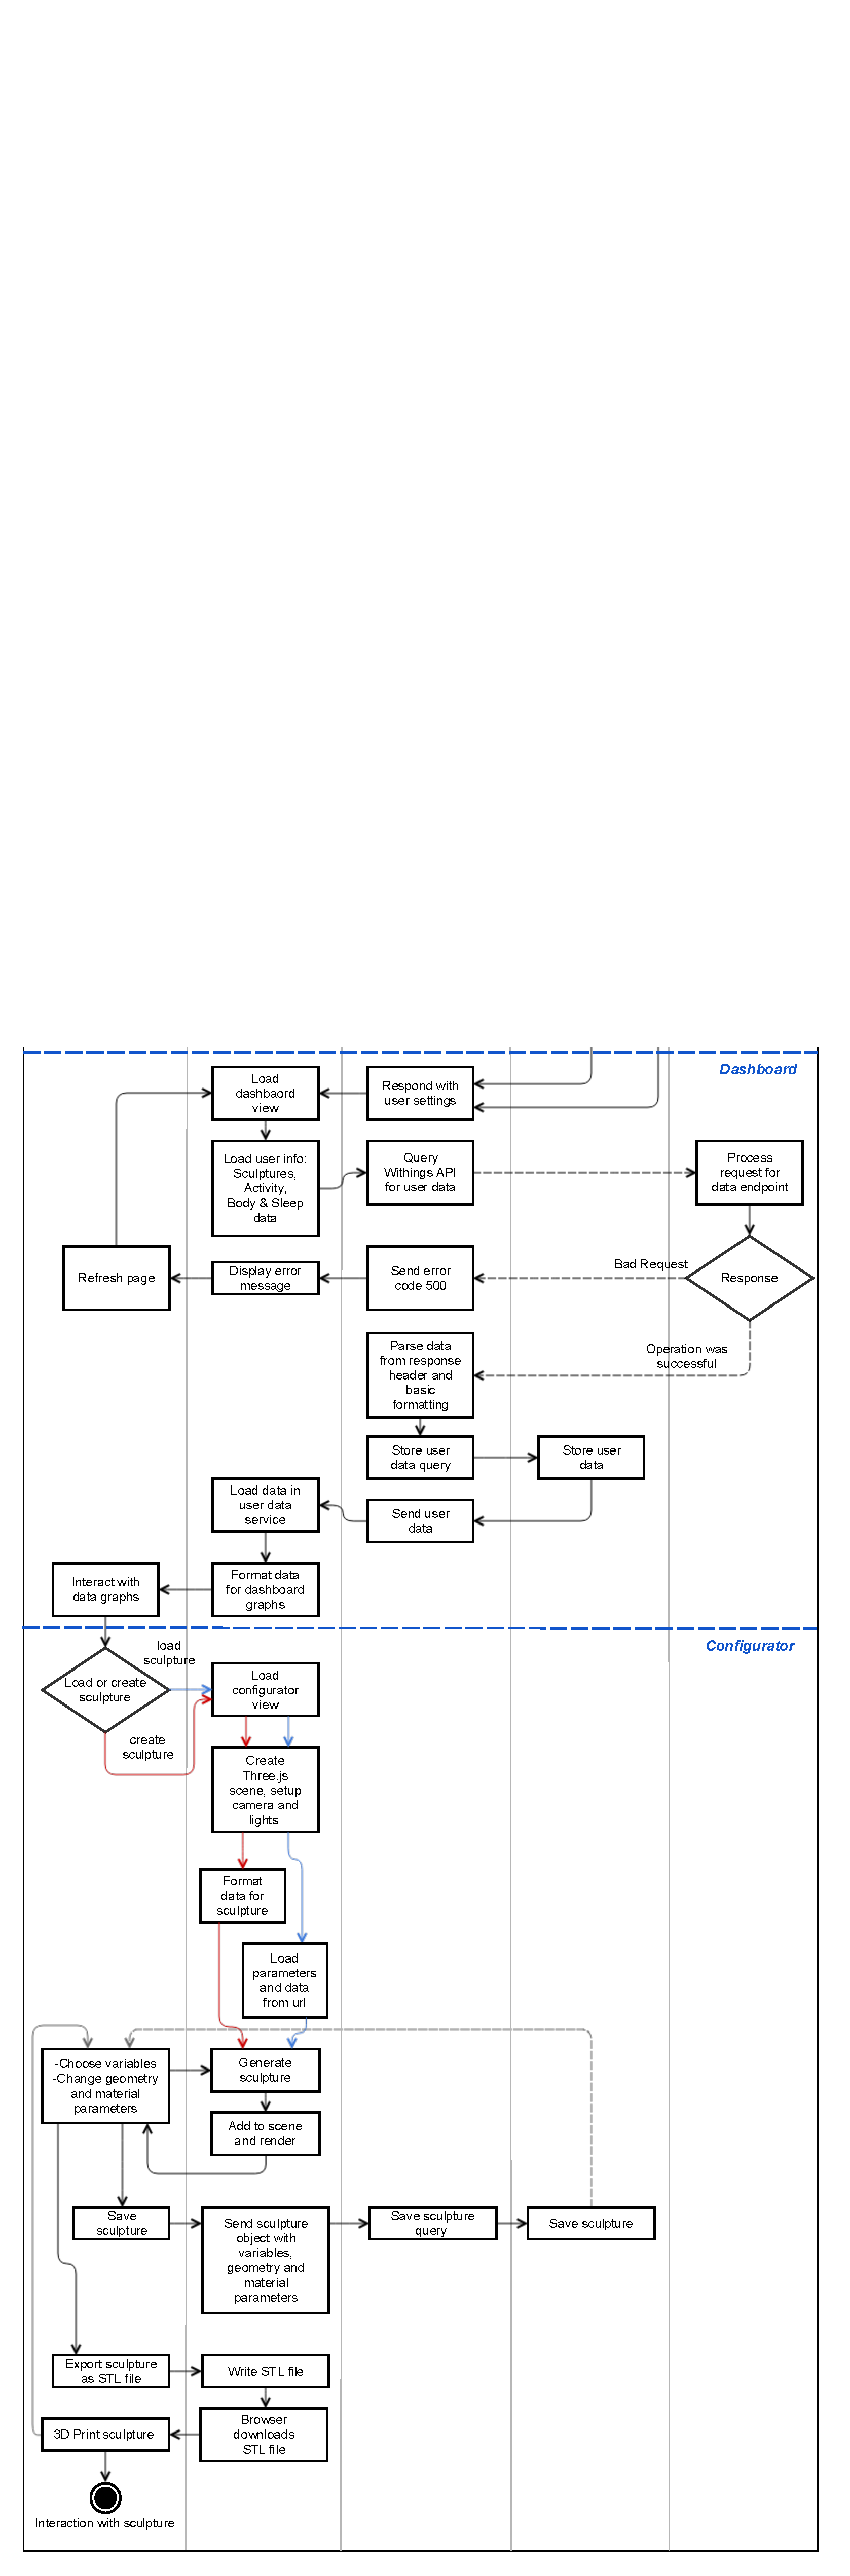
\includegraphics[width=0.82\textwidth]{Configurator/img/flow_diagram_2}
  \caption{Activity Sculpture web configurator's flow diagram part 2}
\label{fig:flowdiagram2}
\end{center}
\end{figure}

\subsection{Configurator}
\subsubsection{Sculpture Generation \& Rendering}


\subsubsection{Sculpture Manipulation}

\label{sub:sculpturegeneration}
\subsection{Backend}
\subsubsection{Withings API Integration}
\label{sub:ApiIntegration}

Authentication 
\textbf{Passport}\cite{passport} 
\textbf{OAuth} \cite{hammer2010oauth}

Querying user data
\textbf{Withings-API}\cite{withingsApi} 



\subsubsection{Data Processing}
\subsection{Challenges}
\end{document}